\thispagestyle{empty}
\chapter{Ruby on Rails}\label{chap:ruby_on_rails}

The \textsf{web application framework}\footnote{
  A web application framework aims to minimize the overhead associated with common activities performed in Web development. 
  For example, it might provide libraries for database access, templating frameworks or session management. 
  It often promotes code reuse.
} Ruby on Rails (Rails) is an excellent example of a successful open source project.
However, we cannot talk about Rails without first talking about the Ruby programming language.

It is a common misconception to confuse Ruby with Ruby on Rails. 
Although closely related, they are distinct things.
When someone says Ruby, it is referring to a programming language.
Ruby on Rails refers to a full-stack framework to develop web applications that was created using Ruby.
Rails helped propel movements like 
Test Driven Development, Pair Programming and other Agile Methodologies, 
and it played a major role in Ruby adoption. 

In this chapter you can read a brief history about the Ruby language
and learn its most distinctive characteristics.
Next, you will find out how Rails turned to be one of the 
most recognized frameworks for developing web applications.
After discussing the main concepts involved in the Rails framework, 
a section is dedicated to the framework structure. 
The chapter ends with a characterizing of the Rails community. 



\section{Ruby Programing Language} 
Ruby is an open source, dynamic and object oriented programming language.
It is not only free of charge, but also free to use, copy, modify, and distribute.
Ruby was created by Yukihiro Matsumoto (also known as \emph{matz}) and public released in 1995, 
it achieved mass acceptance in 2006.

Matsumoto blended parts of his favorite languages (Perl, Smalltalk, Eiffel, Ada, and Lisp) 
balancing functional programming with imperative programming 
to create a multi-paradigm language. 
The objective was to create a \emph{natural} language. 
That does not mean that ruby is simple, Matsumoto often explains the difference by saying:

\begin{quote}\emph{
  Ruby is simple in appearance, but is very complex inside, just like our human body.
}\end{quote}

He believes people want to express themselves when they program. 
Programmers do not want to fight with the language.
Programming languages must feel natural to them.
Ruby is based on "Principle of Least Surprise", 
that means the language behaves the way you expect it to behave.

In Ruby everything is an object. Even basic datatypes, such as numbers or booleans.
Furthermore, every operations in an object is a method and every method returns an object.
A basic rule of the object oriented paradigm is that every object has a class.
So if you call the method class on any object,
it will return another object representing the first object class, 
since this last object is an object too, 
it will also respond to the same method. 
A class object will respond to the method class returning the class object "Class" whose class is itself. 
The class "Class" can be considered a metaclass, because their instances are classes to.
In~\ref{lst:ruby_objects} a simple snippet of ruby code shows this tricky characteristic.
The code can be run in 
\textsf{IRB}\footnote{
  Interactive Ruby Shell (IRB) is a shell for programming in the object-oriented scripting language Ruby.
  It can be launched from a command line and allows the execution of Ruby commands with immediate response, 
  experimenting in real-time.
 },
this tool is of great help for ruby programers,
and an easy way for new comers to start learning.

\begin{rubycode}{Sample Ruby Code}{lst:ruby_objects}
  >> # You can call methods on directly on numbers because they are objects.
  >> 1.to_s
  => "1"

  >> # Everything is an object, and every object responds to the class method.
  >> "1".class
  => String

  >> # Even classes are seen as objects.
  >> "1".class.class
  => Class

  >> # Class is a metaclass. 
  >> "1".class.class.class
  => Class
\end{rubycode}

Ruby is dynamic and interpreted at run time with 
\textsf{duck typing}\footnote{
  Duck typing, in object oriented programing languages, 
  is a style of dynamic typing in which the object methods and properties determine the valid semantics, 
  rather than its inheritance from a particular class or implementation of a specific interface.
} 
"If it walks like a duck and quacks like a duck, then it is a duck!".

Ruby has open classes, this means that at any moment it is possible to change 
any class methods and definitions. That also means that programmers are allowed to change predefined classes.
The truth is that depending on the usage it can be either a good or a bad thing.
Doing some of those things clearly violates the object oriented principle of encapsulation. 
An example of a bad usage would be to 
\textsf{monkey patch}\footnote{
  The term monkey patch means any dynamic modification to a class and 
  is often used as a synonym for dynamically modifying any class at runtime.
} 
the size or length method of string objects to make it not take into consideration white spaces.
It might be useful for a certain situation, 
but it might give a big headache to someone coming to the project few days later.

However, if it was not for those characteristics, 
rails would not have been able to easily change some of ruby basic datatypes and 
consequently developers would not be able to write amazingly readable code like shown in~\ref{lst:ruby_date_calculations}.

\begin{rubycode}{Sample Ruby Code (Rails Environment)}{lst:ruby_date_calculations}
  >> # Calling the method \"today\" on the class \"Date\" 
  >> # returns a date object.
  >> Date.today 
  => Sat, 11 Feb 2012

  >> # It is possible to do calculations on those objects, 
  >> # rails extends the Fixnum class with nice methods to 
  >> # help on those calculations
  >> Date.today + 3.months - 7.day
  => Fri, 04 May 2012
\end{rubycode}

Some of this ruby characteristics are seen by some people as amazing features 
but many careful programers call it "dark magic". In the end, it always comes to the 
good sense of the people writing the code. But with there is no doubt that 
the ruby language has drawn thousands of devoted coders worldwide.
The reason behind that can only be its elegant syntax that is natural to read and easy to write. 
In addition, many of the philosophies that are present in the Ruby on Rails framework,
like "Don't Repeat Yourself" and "Principle of Least Surprise" (we will talk in more detail about that later in this chapter) 
are also shared by Ruby language.
Ruby programs are easy to read and understand, even for a new comer. 
All this makes ruby projects highly maintainable and the programmers using it just fell good.
As its inventor, Matsumoto, concluded in his presentation at the ACM Finals in Japan of 2007: 
\begin{quote}\emph{
  Usability matters, feeling matters. Don't think, feel.
}\end{quote}




\section{Ruby on Rails Framework} 
In 2001, David Heinemeier Hansson was hired by Jason Fried to build a web-based project management tool, 
which ultimately became the 
\textsf{37signals}\footnote{
  37signals is a privately held web application company based in Chicago, Illinois. 
  The firm was co-founded in 1999 by Jason Fried, Carlos Segura, and Ernest Kim.
}
\textsf{Software as a Service}\footnote{
 Software as a service (SaaS) is a software delivery model in which software and associated data are centrally hosted on the cloud.
 Typically, in SaaS, users access software using a thin client via a web browser.
}  
product named 
\textsf{Basecamp}\footnote{
  Basecamp is a web-based project-management tool developed by 37signals and launched in 2004.
}.

He decide to start the project by developing a custom web framework using the ruby programming language
to avoid what he saw as repetitive coding inherent in platforms such as Java,
ruby was almost unknown at the time.

The framework he created was later released as an open source project, separately from the project management tool. 
The name of this open source web framework is Ruby on Rails.

In 2005, Hansson called the attention of the community with a legendary video named "Creating a Weblog in 15 minutes". 
It was an introduction describing how to develop with Rails.
In the same year, his creation earned him the Google-O'Reilly Best Hacker award.
Moreover, the success of Ruby on Rails is considered the biggest responsible for Ruby mass acceptance.

More ruby frameworks were born along the away, 
\textsf{Merb}\footnote{
 Like Ruby on Rails, Merb is an MVC framework built using ruby.
 Unlike Rails 2 (a big framework), Merb adopted an approach that focused on essential core functionality, 
 it was built for speed, leaving extra functionalities to plugins.
}
was one of them.

Nevertheless, on 23th of December, 2008, it was announced
\textsf{(by David in the Rails web site)}\footnote{
 http://weblog.rubyonrails.org/2008/12/23/merb-gets-merged-into-rails-3
}
that Merb would be merged into Rails 3.
This ended unnecessary duplication on both open source communities 
and closed the debate about when to choose one over the other.
The best ideas, from both sides of the fence, were chosen to create a better and stronger project.
This a nice example of how the open source ruby community works. 

This is a nice advantage comparing for instance with the java world, 
where you can find dozens of different frameworks for the same purposes.
Because there is so much choice, developers end-up confused.
In the end, developers are part of different communities. 
It seems like if they are using different languages, most of the time
they cannot try the different options and they do not know which one is better, 
it is just a matter of belief (like a football team).
The problem is that these sub groups might have a common goal but
are paddling in different directions.
Because of that there is less collaboration and the progress is slower.
Although with an incredible exponential grow in the last years,
which might lead to different and new ways of thinking, 
this big divisions does not seams to be happening the rails community.

The Rails philosophy includes several guiding principles:
\begin{itemize}
\item Model-View-Controller (MVC): Rails uses the MVC architecture and 
      is intended to be used with an Agile development methodology,
      providing developers a rapid Web application development environment.
\item Convention over Configuration: Rails makes assumptions about 
      what you want to do and how you are going to do it, 
      rather than letting you tweak every little thing through endless configuration files.
\item Don’t Repeat Yourself (DRY): Writing the same code over and over again is a bad thing. 
      DRY is a principle of software development aimed at reducing repetition of information of all kinds.
\item REST (Representational State Transfer) - A pattern for Web application, 
      organizing your application around resources and standard HTTP verb is the fastest way to go.
\end{itemize}
that will be described with detail in following sections.


\section{Model-View-Controller} 
MVC is an architectural pattern used in software engineering. 
Successful use of the pattern isolates business logic from user interface considerations, 
resulting in an application where it is easier to modify either the visual appearance of the application 
or the underlying business rules without affecting the other.
MVC was first described in 1979 by Trygye Reenskaug.

\begin{figure}[h!]
  \caption{Model-View-Controller Diagram}
  \centering
  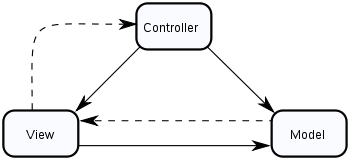
\includegraphics[width=0.5\textwidth]{Images/ModelViewController}
\end{figure}

\begin{itemize}
\item A \emph{model} represents the information of the application and the rules to manipulate that data. In Rails, models are used for managing the rules of interaction with a corresponding database table. In most cases, one table in your database will correspond to one model in your application. Your application logic will be concentrated in the models.
\item A \emph{view} represents the user interface of your application. In Rails, views are often HTML files with embedded Ruby code (which we call erb templates) to perform tasks related to the presentation of the data. Views handle the job of providing data to the web browser or other tool that is used to make requests to your application.
\item \emph{Controllers} provide the “glue” between model and views. In Rails, controllers are responsible for processing the incoming requests from the web browser, interrogating the models for data, and passing the data to the views for presentation.
\end{itemize}

The benefits of using MVC include the isolation of business logic from the user interface.
In addition it becomes easier to keep the code DRY and 
it makes clear where different types of code belong for easier maintenance.



\section{Convention over Configuration} 
Traditionally, frameworks need multiple configuration files, each with many settings. 
These provide information specific to each project, ranging from URLs to mappings between classes and database tables. 
With the complexity of an application, the size and number of those files grows as well. 
Most of the time it is very hard to maintain a lot of configurations files. 
Rails was developed to minimize these issues by following the \emph{Convention over Configuration} paradigm.

\emph{Convention over Configuration} aims at simplifying the development without losing the application flexibility. 
It means you do not need to write configuration files to have a flexible application. 
This leads to less code and less repetition.
The Rails creator calls this “Intelligent Patterns”. 
If you do not want to configure anything, just follow the conventions and the framework will know what to do.

To better understand \emph{Convention over Configuration}, 
let's see how Rails analyses a URL such as the following:

\begin{rubycode}{URL Example}{lst:rails_url}
  /account/show/1

\end{rubycode}
By default, the framework will split the URL by “/” and following the rest standards 
we can expect a few things to be true: 

\begin{itemize}
\item \emph{account} – It probably means that a controller called “AccountController” exists in the application. It should be a class that extends the ApplicationController class and handles all kind of actions related with accounts.
\item \emph{show} – The AccountController class should have a show method, 
this method will probably interact with a model called Account to fetch the needed data and pass it to a view, 
which will render a nice page showing the account information.
\item \emph{1} – Since we are in the accounts show action this is the parameter called “id” with the value “1”. 
It means that user want to see information about the account whose id is 1. 
\end{itemize}

Although, it is fairly easy to change this behavior (in fact, it is a best practice to change it a little bit), 
without writing one line code, a rails application freshly created expects all those things, 
we just need to create the controller, a view, and have a database, with the correct names and everything works by itself. 
In many others frameworks it is necessary to create one or more configuration files, normally XML files.

Another example of \emph{Convention over Configuration} is with respect to the persistence layer 
(which typically deals with a database). 
The only thing you need to do in order to map a Model to its table in the database is 
the code shown in~\ref{lst:rails_product_model}.
\begin{rubycode}{Sample Model file “product.rb”}{lst:rails_product_model}
class Product < ActiveRecord::Base 
end
\end{rubycode}

That is enough for the class to be bound by the framework with a table in the database called Products and all of its columns will be accessible for use without creating a configuration file to map it. Note as well that you do not need to create getter and setter methods but they will be there ready to use.
Rails has a concept of pluralize, which means a model Product will have a table Products in the database, or a model Customer will have a table Customers and so on.



\section{Don’t Repeat Yourself} 
Don’t Repeat Yourself (DRY) is an approach aimed at reducing duplication. 
The philosophy emphasizes that information should not be duplicated, 
because duplicates increase the difficulty of code maintenance, 
decrease clarity and lead to opportunities for inconsistencies.

DRY is applied quite broadly to include database schemas, 
test plans, the build system, and even documentation. 
When the DRY principle is applied successfully, 
a modification of any single element of a system does not change other logically-unrelated elements.
DRY code is created by data transformation, which allows the software developer to avoid copy and paste operations.
DRY code usually makes large software system easier to maintain, 
as long as the data transformations are easy to create and maintain.
DRY is not about just avoiding code duplication, 
but more generally about avoiding multiple and possibly diverging ways to express every piece of knowledge: 
e.g., logic, database schemas, and constants.
If we are always repeating the same code, 
refactoring will be in order to keep your code DRY compliant. 



\section{The Framework Structure} 
Every Rails application follows the same file structure organization. 
This way everything should be in the right spot.

After generating a new Rails application 
(this is achieve by running just the single command line shown in Listing~\ref{lst:new_rails_app} ) 
\begin{rubycode}{Command to create a new rails application}{lst:new_rails_app}
  rails new <name_of_the_appliction>,

\end{rubycode}
a folder looking like the tree in Figure~\ref{fig:rails_file_structure} should be created. 
It is a ready to run web application.

The folder called \emph{app}, 
is where the majority of the real code for the new application goes (models, views, controllers, helpers, etc).
The other folders are usually destined to documentation, configuration, third party code, temporary files, etc.

\begin{figure}[h!]
  \caption{Rails Project File Structure}\label{fig:rails_file_structure}
  \centering
  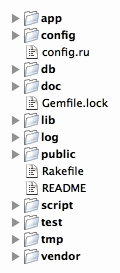
\includegraphics[scale=0.75]{Images/rails_files}
\end{figure}

Rails is a \textsf{meta-framework}\footnote{
  A meta-framework is a framework composed of smaller frameworks.
}, it is composed of the following frameworks:


\subsection{Active Record}
Active Record connect business object and database tables to create a persistable domain model where logic and data are presented in on wrapping. It’s an implementation of the object-relational mapping (ORM) pattern by the same name as described by Martin Fowler.
Active Record is the base for the models in a Rails application.

It provides database independence, basic CRUD (Create, Read, Update, and Delete) functionality, advanced finding capabilities, and the ability to relate models to one another, among other services.


\subsection{Action Pack} 
Action Pack splits the response to a web request into a controller part (performing the logic) and a view part (rendering a template). This two-step approach is known as an action, which will normally create, read, update, 
or delete some entity defined by a model (often backed by a database) 
before choosing either to render a template or redirecting to another action.

Action Pack implements these actions as public methods on Action Controllers and uses Action Views to implement the template rendering. Action Controllers are then responsible for handling all the action relating to a certain part of an application, 
like listing, creating, deleting, and updating records.

Action View templates are written using embedded Ruby in tags mingled in with the HTML. 
To avoid cluttering the templates with code, a bunch of help classes provide common behavior for forms, dates, and strings. 
And it is easy to add specific helpers to keep the separations as the application evolves.


\subsection{Action Mailer}  
Action Mailer is a framework for building e-mail services. You can use Action Mailer to send emails based on flexible templates, or to receive and process incoming email.


\subsection{Active Support} 
Active Support is an extensive collection of utility classes and standard Ruby library extensions that are used in the Rails. 
All these additions have hence been collected in this bundle as way to gather all that sugar that makes Ruby sweeter. 
For instance, the examples shown previously regarding date and time calculations are part of this bundle.


\section{Rails Community} 
The biggest part of Ruby developers are in fact Rails developers. 
Moreover, Rails is considered the biggest responsible for Ruby popularity
(tens of thousands of Rails applications are online).
In addition, Rails developers are also web developers, 
so we can assume that the majority of Ruby and Rails developers also write HTML, javascript and CSS.
The Ruby and Ruby on Rails community has been growing up in the last years. 
Programmers from other languages like Java, .NET are discovering the power of Ruby and how easy is 
to create web application using Rails.

Ruby and Ruby on Rails community members love conventions and best practices.
It is also common to associate Ruby on Rails with Behaviour Driven Development (BDD) and Agile methodologies.
For instance, a lot of Ruby on Rails book authors speak about automated tests, 
written using domain specific languages (DSLs), like Cucumber or Rspec, 
this might seam advanced stuff, but writing automated tests in Ruby is fairly easy,
and of course DSLs like Cucumber and Rspec follow the human/natural philosophies of ruby.

In ~\ref{lst:cucumber}, a simple Cucumber test file shows how readable Cucumber tests can be.

It looks like a use-case, but this is a real automated test, 
by using the power of regular expressions and ruby dynamic capabilities
it is possible to parse this Cucumber file and check if the software is valid according to the specification. 

\begin{rubycode}{Cumber feature}{lst:cucumber}
Feature: Search courses
  Potential students should be able to search for courses

  Scenario: Search by topic
    Given there are 34 courses which do not have the topic "math"
    And there are 2 courses LEI, MEI that each have "math" as one of the topics
    When I search for "math"
    Then I should see the following courses:
      | Course code |
      | LEI         |
      | MEI         |
\end{rubycode}

There are a lot of open source projects, frameworks and communities. 
However, like it was shown during this chapter, the characteristics of Rails and the various philosophies underlying it,
makes this community of great potential to be a starting point to understand the role of best practices, 
its benefits and how to measure it. 

Later in this document, we will identify which ones are the most relevant Rails best practices,
and discover if the projects that do follow best practices are truly the projects with more success in the community.

